%%
%% Copyright 2007, 2008, 2009 Elsevier Ltd
%%
%% This file is part of the 'Elsarticle Bundle'.
%% ---------------------------------------------
%%
%% It may be distributed under the conditions of the LaTeX Project Public
%% License, either version 1.2 of this license or (at your option) any
%% later version.  The latest version of this license is in
%%    http://www.latex-project.org/lppl.txt
%% and version 1.2 or later is part of all distributions of LaTeX
%% version 1999/12/01 or later.
%%
%% The list of all files belonging to the 'Elsarticle Bundle' is
%% given in the file `manifest.txt'.
%%

%% Template article for Elsevier's document class `elsarticle'
%% with harvard style bibliographic references
%% SP 2008/03/01
%%
%%
%%
%% $Id: elsarticle-template-harv.tex 4 2009-10-24 08:22:58Z rishi $
%%
%%
\documentclass[final,authoryear,11pt,times]{elsarticle}

%% Use the option review to obtain double line spacing
%% \documentclass[authoryear,preprint,review,12pt]{elsarticle}

%% Use the options 1p,twocolumn; 3p; 3p,twocolumn; 5p; or 5p,twocolumn
%% for a journal layout:
%% \documentclass[final,authoryear,1p,times]{elsarticle}
%% \documentclass[final,authoryear,1p,times,twocolumn]{elsarticle}
%% \documentclass[final,authoryear,3p,times]{elsarticle}
%% \documentclass[final,authoryear,3p,times,twocolumn]{elsarticle}

%% \documentclass[final,authoryear,5p,times,twocolumn]{elsarticle}

%% if you use PostScript figures in your article
%% use the graphics package for simple commands
%% \usepackage{graphics}
%% or use the graphicx package for more complicated commands
%% \usepackage{graphicx}
%% or use the epsfig package if you prefer to use the old commands
%% \usepackage{epsfig}

%% The amssymb package provides various useful mathematical symbols
\usepackage{amssymb}

\usepackage[margin=1.25in]{geometry}
\usepackage{bbm}
\usepackage{float}
\usepackage{graphicx}
\usepackage{caption}
\usepackage{subcaption}
\usepackage{cleveref}
\usepackage{csquotes}

\usepackage{setspace}
\onehalfspacing
\usepackage{hyperref}
\hypersetup{
    colorlinks=true,
    linkcolor=blue,
    filecolor=magenta,      
    urlcolor=cyan,
}
\urlstyle{same}

\captionsetup[subfigure]{subrefformat=simple,labelformat=simple}
\renewcommand\thesubfigure{(\alph{subfigure})}

%% The amsthm package provides extended theorem environments
%% \usepackage{amsthm}

%% The lineno packages adds line numbers. Start line numbering with
%% \begin{linenumbers}, end it with \end{linenumbers}. Or switch it on
%% for the whole article with \linenumbers after \end{frontmatter}.
%% \usepackage{lineno}

%% natbib.sty is loaded by default. However, natbib options can be
%% provided with \biboptions{...} command. Following options are
%% valid:

%%   round  -  round parentheses are used (default)
%%   square -  square brackets are used   [option]
%%   curly  -  curly braces are used      {option}
%%   angle  -  angle brackets are used    <option>
%%   semicolon  -  multiple citations separated by semi-colon (default)
%%   colon  - same as semicolon, an earlier confusion
%%   comma  -  separated by comma
%%   authoryear - selects author-year citations (default)
%%   numbers-  selects numerical citations
%%   super  -  numerical citations as superscripts
%%   sort   -  sorts multiple citations according to order in ref. list
%%   sort&compress   -  like sort, but also compresses numerical citations
%%   compress - compresses without sorting
%%   longnamesfirst  -  makes first citation full author list
%%
%% \biboptions{longnamesfirst,comma}

% \biboptions{}
% \setlength{\parskip}{1em}

\journal{cs280r - Final Project Report}

\begin{document}

\begin{frontmatter}

%% Title, authors and addresses

%% use the tnoteref command within \title for footnotes;
%% use the tnotetext command for the associated footnote;
%% use the fnref command within \author or \address for footnotes;
%% use the fntext command for the associated footnote;
%% use the corref command within \author for corresponding author footnotes;
%% use the cortext command for the associated footnote;
%% use the ead command for the email address,
%% and the form \ead[url] for the home page:
%%
%% \title{Title\tnoteref{label1}}
%% \tnotetext[label1]{}
%% \author{Name\corref{cor1}\fnref{label2}}
%% \ead{email address}
%% \ead[url]{home page}
%% \fntext[label2]{}
%% \cortext[cor1]{}
%% \address{Address\fnref{label3}}
%% \fntext[label3]{}

\title{CS280r Final Project Report \\ Voting Rules for Subset Selection}

%% use optional labels to link authors explicitly to addresses:
%% \author[label1,label2]{<author name>}
%% \address[label1]{<address>}
%% \address[label2]{<address>}

\author{Anna Sophie Hilgard and Nicholas Hoernle}


\begin{abstract}
\textit{
Social choice theory, providing tools for making joint decisions in multi-agent systems is becoming popular for tasks such as group recommendation systems, information retrieval, and crowdsourcing \citep{moulin2016handbook}. We pose a scenario where a crowd is asked to select a subset of information points regarding a topic and we show that theoretically optimal voting rules are not necessarily applicable to this setting. Rather, we suggest different voting rules place varying amounts of cognitive load on the participants, introducing noise into the votes of the participants and ultimately confounding the results. Our conclusion is that cognitive load on the voter and separability of the voting points should be included as modeling variables for voting rules that involve subset selection.}

\end{abstract}
\end{frontmatter}

% \linenumbers

%% main text
\section{Introduction}
\label{sec:introduction}
There are interesting settings where humans collaborate with each other and with computers to generate content, including documents (Wikipedia, inter alia) \citep{hahn2016knowledge,kittur2013future}, taxonomies \citep{chilton2013cascade} and summaries \citep{khosla2013large}. In multi-agent settings where qualitative content is being created or used, it is important to consider the negative consequences of too much communicative noise. Given a medical setting, \citet{amir2015care} report that study participants could not review necessary information in a timely manner, nullifying the effect of obtaining complete and correct information from others. \citet{hahn2016knowledge} show that crowdsourcing vendors consistently struggle to balance the amount of information needed to convey to a worker to equip the worker to excel at his/her job without overburdening the process with too much information. 

An added complication is that in many settings, the ideal contextual information to be shared is subjective, and multiple parties have competing interests in having their contributions addressed. One possible solution is to allow for a single contributor or an outside controller to make these subjective decisions. However, experiences with content generators with a strong hierarchical or dictatorial leadership \citep{benkler2015peer} have shown that the resulting content is often suboptimal from the viewpoint of the whole and heavily skewed to conform to the opinion(s) of the decision-maker(s). 

% \subsection{Motivation for Investigation}
% \label{sec:motivation}
Under these conditions, there is a strong case for adopting social budgeting techniques to crowdsource contextual points. Our ultimate goal is to select an ideal set of relevant contextual information while reducing the communication and collaboration overheads that may otherwise be necessary. \citet{schwartz2015design} stresses that collective assessment is most critical in heterogeneous environments in which group members have different information and the actions of individuals are interdependent. In such an environment, an algorithm that satisfies the criterion of representativity, such that the composition of the final selection represents the will of all of the voters, will be more globally favorable than an algorithm that simply maximizes total utility \citep{moulin2016handbook}. Such algorithms are those that minimize the worst case outcomes over all voters. 

In a context in which there exists a rank order of preferences, the poorness of an outcome for any given voter is evaluated to be the rank of the highest ranking object in his or her rating which appears in the selected subset. That is, the extent of the misrepresentation of an agent is the number of his or her preferred options that were not selected.

\section{Related Work}
\citet{boutilier2015optimal} show that in such a utilitarian framework in which we hope to maximize the satisfaction of all group members, properly chosen voting aggregation rules can ensure that a subset is selected which minimizes the maximum difference between the optimal possible satisfaction to all members and the satisfaction of the subset selected by the voting rule in expectation.  This difference is hereafter referred to as regret. In particular, we will seek to test the effectiveness of the subset selection algorithm generated by \citet{caragiannis2017subset}, which approaches the problem as a variation on the maximin rule. The authors show that it is possible to derive an explicit utility function which maximizes regret while maintaining consistency with the votes. The following expression is used for maximum regret for a subset selection $T$:
\begin{equation}\label{eq:max_regret}
\textrm{max}_{S \in A_k} \sum_{i=1}^{n} \frac{\mathbbm{1}[S \succ_{\sigma_i}T]}{\sigma_i(S)}
\end{equation}
where $S \succ_{\sigma_i}T$ indicates that there is no alternative in T preferred to every alternative in S given the utility function $\sigma_i$. $\sigma_i(S)$ is the ordinal ranking of the best alternative in set $S$ in the ranking determined by the utility function $\sigma_i$. Intuitively, any term in this maximization captures the lost satisfaction to the voters of not having the given set $S_i$ chosen rather than $T$, weighted by how much he or she liked his or her best option in $S_i$. This will lead to a greater penalization for sets $T$ that do not give many participants at least one of their top choices. We seek the set $T$ that minimizes this quantity.
\begin{equation}\label{eq:min_regret}
\textrm{argmin}_{T \in A_k} \textrm{max}_{S \in A_k} \sum_{i=1}^{n} \frac{\mathbbm{1}[S \succ_{\sigma_i}T]}{\sigma_i(S)}
\end{equation}

\citet{caragiannis2017subset} show that equation \ref{eq:min_regret} can be solved through an integer linear program (ILP) with $n � m$ variables and $n � m^{2} + {n\choose m}$ constraints, where $n$ is the number of voters and $m$ is the number of alternatives available.

For comparison, we also consider plurality/knapsack voting, which has been used in real-world participatory budgeting programs (likely in part because of its computational simplicity and ease of understanding \citeauthor{goel2015knapsack}). Moreover, in spite of not directly optimizing for minimum regret, plurality is shown by \citet{caragiannis2017subset} to have an empirical upper bound on regret approaching that of the subset selection algorithm above (\ref{eq:min_regret}) for subset sizes greater than three, which will be the case in our experiment and should be generally true for problems of this nature. We additionally provide two interfaces for the ranking problem, one in which users directly sort the subset, and one in which users rate each point in a subset, and a ranking is induced over the ratings before aggregation. This allows additional investigation of the problem of cognitive load in voting systems.

%We apply these different voting rules to the problem of subset selection and conclude that in practice the success of a voting rule may depend heavily on the difficulty (cognitively or subjectively) one has in comparing options. 

%Definition 1 (Comparing Sets). Given a ranking ? ? L and an alternative a ? A, recall that ?(a) denotes the position of a in ?. More generally, for a set S ? A let ?(S) = mina?S ?(a). For sets S,T ? A, we say T ?? S if ?(T) < ?(S), i.e., if there exists an alternative in T that is preferred to every alternative in S in ?.

%The need for such efficient communication was evi- dent in our study: some of the providers we interviewed re- ported that when complete plans or notes are sent to them, they are unable to determine the information most important to consider, and they do not review the information in a timely manner as a result of this information overload. 

%Previous crowdsourc- ing approaches have trouble dealing with cross-topic consis- tency because reading even a single topic can take significant time, let alone reading and editing across all topics.

%These are often ones in which
%individuals must coordinate their actions because their parts of the organization are
%interdependent.

%Correctly specifying an agenda helps to keep meeting topics on track, on time and helps to improve the efficiency and effectiveness of the meeting \citep{schwartz2015design} \citep{lehmann2013sequential}. \citet{schwartz2015design} continues by stating the importance of including items in the agenda that reflect the needs of the individuals in the team. \citet{lehmann2013sequential} assert that unmanaged social interaction leads to poor decision making, ineffective communication and unnecessary conformity. In this light, we have revisited the Care Coordination work presented by \citet{amir2015care} and focus on designing a human-computer collaboration tool that is able to manage the creation of an agenda that is relevant for a diverse team of individuals. \citep{arber2008team} is in agreement with the thesis here that meetings significantly affect the performance of the medical team and on the care that the patient receives. The purpose of this system is to extend \citet{procaccia2016voting} `Voting Rules' framework and text mining techniques to create an initial set of structured agenda items that can then be agreed upon in advance. Furthermore, some of the specific obstacles to efficient teamwork demonstrated in the \citet{amir2015care} study shows that members of the team often find large meetings unproductive and not related to the work that they are doing with the patient. Having a structured agenda in advance will help the team members filter through the potentially time wasting and irrelevant content such that they can address the pertinent issues at hand. Following \citet{schwartz2015design} framework for creating an effective meeting agenda, we propose an agent that is able to source the relevant agenda items, action points and required duration from the team prior to the meeting occurring.
%
%\citep{fatima2004agenda} present a view of negotiations where agents all benefit by reaching an agreement but all have conflicting ideas over how certain tasks should be executed. In a similar way, agents in \citet{amir2015care} medical setting may have differing opinions on the best and most important treatment plans that require discussion, but reaching a feasible agreement in advance... 

\section{Experiment Design}
\label{sec:experiment}
Three voting rules are compared to evaluate the success of the subset selection. To test the voting rules, we pose a setting where participants are requested to select a number of points that may be relevant to a given topic. We compiled a set of 10 supporting points from popular \textit{New York Times} opinion pieces and used a web-based survey form to allow participants to make subset selections. The topics were presented in a `debate prompt' style and the participants were asked to select the points that would contribute the most value to the presented argument. We also allowed participants to provide feedback on the subset selection styles that they most and least enjoyed (\ref{appendix:qual_feedback}).

\par The interface\footnote{Accessed at: \url{http://nick-and-sophie-harvard-cs280r.s3-website-us-east-1.amazonaws.com/index.html}} was designed to present participants with three topics (corresponding to the three articles) and each topic with a different subset selection algorithm for different contextual points relating to the topic. The different selection methods include:
\begin{itemize}
\itemsep0em 
\item `ranking' by dragging and dropping alternatives into the correct order from most to least useful for the given argument. 
\item `cardinal' rating where each point was given a score out of 10 independently of the others.
\item `plurality' (or knapsack) selection, where check-boxes were selected until 5 selections were made.
\end{itemize}

The study consisted of 37 respondents, each with three subset choices over the three different voting rules (they are presented with one option for each rule). We solve equation \ref{eq:min_regret} using integer linear programming as described by \citet{caragiannis2017subset} to aggregate the ranking and cardinal results into an optimal subset. We induced a ranking over the cardinal results to obtain ranked values to use in the subset selection algorithm, breaking ties at random. For the plurality results, we selected the subset greedily using a majority rule approach. Selected subsets included four points each.

Finally, selected subsets were presented to a different group of 17 participants. These participants were simply asked to select the most relevant subset, given the same topic. This data was also collected through a web-based survey \footnote{Accessed at: \url{http://nick-and-sophie-harvard-cs280r.s3-website-us-east-1.amazonaws.com}}.


\section{Results} 

The results here, while indicative of trends, are mostly not statistically significant and thus we do not make \textit{significant} claims about our conclusions. Rather, we use the results to pose interesting insights and to inform further work in this area.

The initial results show a large amount of noise and uncertainty in the selections. Figure \ref{fig:q3raw} shows the score that each answer receives for the third topic \footnote{See \ref{appendix:question_topics} for more details on the specific topics} in the question set under the different voting rules. Table \ref{tbl:voting_aggregation} shows the summary of the selected subsets by the voting aggregation rules explained in \ref{sec:experiment}. Points selected by the various methods showed a generally low degree of overlap. For two of the topics, there was one point present in all three subsets, and for all of the topics, at least two points appeared in multiple subsets. Only one pair of options differed by only a single option.  

\begin{figure}
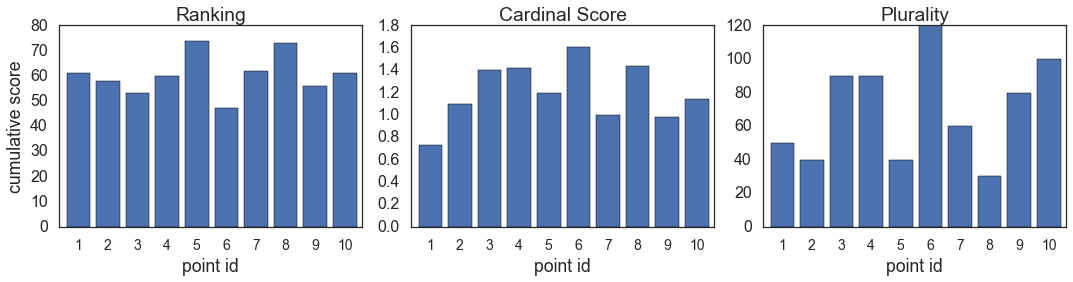
\includegraphics[width=\textwidth, height=4cm]{images/question3_raw_results}
\caption{Bar chart of the score each answer point receives under the different voting rules. Note that for Ranking and Cardinal Score, highest bars do not necessarily correspond to selected points due to the minimum regret objective.}
\label{fig:q3raw}
\end{figure}

\begin{table}
\begin{center}
\begin{tabular}{ l | c | c | c }
 & Topic 1 & Topic 2 & Topic 3 \\
 \hline
 \textbf{Ranking}&              $[2, 3, 6, 7]$ & $[2, 3, 7, 10]$ & $[3, 5, 7, 10]$ \\
 \textbf{Cardinal Score}&       $[1, 2, 7, 8]$ & $[4, 7, 8, 10]$ & $[3, 4, 6, 8]$ \\
 \textbf{Plurality Selection}&   $[1, 5, 7, 9]$& $[1, 2, 3, 8]$  & $[3, 4, 6, 10]$ \\
\end{tabular}
\caption{Table showing the selected subset for the different topics for the different voting rules. }
\label{tbl:voting_aggregation}
\end{center}
\end{table}

A different set of voters was asked to vote on what was qualitatively the best subset. Figure \ref{fig:final_res} shows that the subset from plurality voting produced the most preferred results in all three topics, although for Topic 1 the cardinal score was also tied for the most number of votes. The success of simple plurality voting in our experiment over more complicated minimum regret methods leads to a discussion of the appropriateness of minimum regret in our setting. 

\begin{figure}
\centering
\begin{minipage}[t]{.3\textwidth}
		\centering
		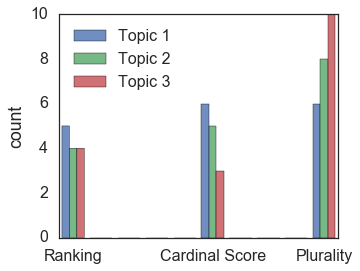
\includegraphics[height=4cm]{images/final_results}
		\caption{Bar chart showing the final count of votes in survey 2 after each subset was selected from survey 1 using the different subset selection algorithms.}
		\label{fig:final_res}
  \label{fig:sub1}
\end{minipage}
\hfill
\begin{minipage}[t]{.3\textwidth}
		\centering
		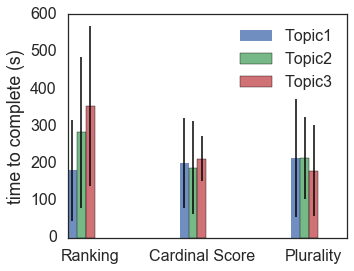
\includegraphics[height=4cm]{images/time_to_complete_raw}
		\caption{Time to complete the different voting sections.}
		\label{fig:time_to_complete}
\end{minipage}
\hfill
\begin{minipage}[t]{.3\textwidth}
		\centering
		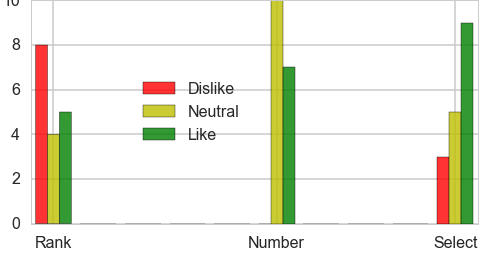
\includegraphics[height=4cm]{images/qualitatve_feedback_responses}
		\caption{Chart showing the qualitative sentiment towards the different voting rules.}
		\label{fig:qualitative_feedback}
\end{minipage}
\end{figure}


The time that it took the participants to complete each voting section was recorded. For Topics 2 and 3, the Ranking vote section took on average 1 minute 30 seconds more time to complete than Cardinal and Plurality voting. However, the results from Topic 1 are inconclusive and the standard deviation on the times is large.

Finally, we turn to the qualitative results that were collected in the initial survey. Here we specifically asked participants to provide feedback on the difficulty of the voting rule, and which voting rules they preferred. An example of this feedback is: \textit{``Ranking is the most difficult. I prefer the format that lets me choose on a scale from 1-10 how strong I think the argument is.''}\footnote{All the qualitative feedback is provided in \ref{appendix:qual_feedback}} We parsed the qualitative feedback to understand the sentiment towards the different voting rules. When a specific voting format was mentioned positively or negatively, this was recorded with a $1$ or $-1$ respectively. If the voting rule was not mentioned or was mentioned in a neutral setting, the score was recorded as 0. Figure \ref{fig:qualitative_feedback} demonstrates a trend where `ranking' was disliked more than it was liked, `plurality' was liked more than it was disliked and `cardinal score' shows a neutral-to-positive sentiment.
\section{Discussion}
The preference for a cardinal over an ordinal method runs counter to generally accepted voting design principles, we believe this may have to do with the number of points that must be considered for any given decision as well as some degree of user frustration at inability to assign ties in the ranking. In particular, to properly rank any adjacent pair of points, the user must consider the value of both at once. In assigning a cardinal ranking, the user can focus only on determining the value of a single point.

The results from \citet{caragiannis2017subset} suggest that for a subset of size four, the minimum regret aggregation algorithm should generally provide the lowest upper bound on the regret of participants. That is, it is better in the case where we assume the utility function with highest possible distortion compatible with the selections. However, plurality voting has a very similar upper bound for a subset size of four and may have superior properties in other considerations, as we've seen above. We believe the success of plurality voting in our experiment has to do with three factors. The first factor is simply that the test group was likely of a more homogeneous makeup than the original subset generation group.\footnote{Given that we had already placed the original survey on social media channels, we relied largely on in-person survey collection and the CS280r course to answer the second survey} The other two factors are discussed below.
\subsection{Utility Functions and Separability}
First, the upper bounds assume the worst case separable utility function compatible with the reported rankings. Even in the case where the utility function is in fact separable, this does not imply anything about the average case, and the two worst case bounds are so similar that it is probable that the average case regret for plurality is in fact better. Furthermore, while the points were selected with the quality that they each could stand alone, we see evidence in the data that respondents may be `bundling' points, leading to a different type or problem entirely, and one for which the utility function used in minimum regret is a poor representation of the true utility of voters. Plurality, too, is susceptible to voting paradoxes with nonseparable utility as seen in \citet{moulin2016handbook}. However, in our case it seems reasonable that the separability assumption is approximately true (in that some points may be slightly complementary but the addition of a point should never be detrimental in the presence of other points), and so plurality yields a reasonable approximation of the optimal answer. 

To investigate the presence of this effect in our collected data, we ran a window of length three over every person's choices, calculating the pairwise distance between all combinations of the three in that window in terms of their identity numbers in our original problem formulation. Because the points were extracted in order from the original opinion pieces (although points are displayed in random order to respondents), numerically close IDs correspond to physical and contextual closeness in the original argument. From this, we get an idea whether points that are similar typically get placed with a similar ranking. Figure \ref{fig:pairwise_distance} shows a strong preference for bundling contextually similar points, even though those points are not displayed together in the experiment. In general, \citet{moulin2016handbook} suggests that in fact there are very few domains in which the separability assumption can be expected to hold. In our experiment in particular, it seems likely that human nature pushes respondents to choose a cohesive argument: that is, one in which the arguments made flow well together. The high frequency of a distance of `1' in the figure \ref{fig:pairwise_distance}, corresponding to users selecting points that semantically occurred next to each other in the original article, are all significant with p-values less than 0.003 when compared to the expected count of `1' given a randomized ordering of the IDs.

Much work has been done to show the failure of voting algorithms designed with the assumption of separability to specific pathological cases in which the assumption does not hold \citep{moulin2016handbook}. However, it is unclear how this lack of general robustness relates to the average performance of the algorithms under varying degrees of violations of the separability assumption, represented here by correspondence between points. 

\begin{figure}
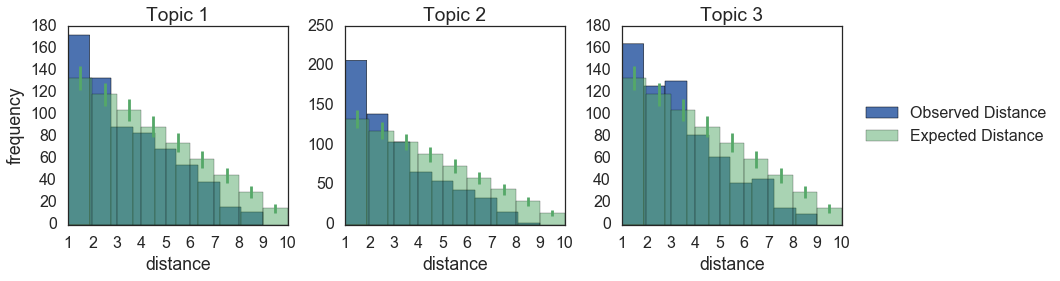
\includegraphics[width=\textwidth, height=4cm]{images/pairwise_distance}
\caption{Counts of distances of points in original article when selected in the top or bottom 5 selections.}
\label{fig:pairwise_distance}
\end{figure}


\subsection{Cognitive Load}
Second, our qualitative feedback suggests that knapsack/plurality selection is significantly easier for respondents. This leads us to consider the possible effects of cognitive load on the various voting algorithms. In fact,  \citeauthor{caragiannis2017subset} explicitly mention that the analysis has yet to investigate effects of cognitive load although the authors stress in other works, such as \citet{benade2017preference} that the entire point of voting mechanisms is to reduce the unacceptable cognitive load of eliciting a full utility function. 

One good reason to do this is that people are likely to make mistakes when presented with a large cognitive load. In particular, in the Sushi dataset from \citet{kamishima2003nantonac}, 70\% of rankings and ratings of the same subsets contain contradictions. That is, the cardinal values in the rating set do not map to the ordinal values in the ranking set. Then it can be assumed that respondents have reported erroneous preferences in one of the two cases, possibly due to excessive cognitive load of the reporting mechanism. If it can be expected that voters will occasionally make errors in reporting their preferences, we should also be interested in the robustness of these selection algorithms to errors. Previous work has shown that the worst case robustness of both minimax and plurality voting is generally better than many other voting methods when considering the worst case for a single winner and that the worst case for a larger subset is bounded by the worst case for a single winner \citep{procaccia2007robustness}. Here, we consider the empirical average case for a variety of subset sizes.

To set up the experiment, we take the Sushi dataset mentioned above and calculate for the rating and ranking problems on the same subsets (these are `sushi3b.5000.10.order' and `sushi3b.5000.10.score') the minimum number of flips of adjacent rankings required to bring the ranking into agreement with a ranking induced over the ratings (flips corresponding to equally rated items are not included in the count, as either ranking of such items is consistent with the rating assuming randomized tie breaking). We tally the distribution of the number of errors throughout all 5000 respondents to the sushi survey. Then, we use the third sushi dataset, `sushi3a.5000.10.order', which contains only 10 types of sushi rather than the 100 in other subsets to bootstrap voting profiles. Because each of the users in the 100 sushi dataset were each only presented with 10 sushi out of the 100, we feel it is fair to assume the same cognitive load would be true for only 10 total sushi types. However, using this dataset allows us to simulate voting over a set of only 10 objects. To create the profiles, we repeatedly draw a set number of voting profiles at random from the rows of the file. We create 100 of these voting profile sets for each trial. Then, we loop through each item in each of the profile sets and induce a number of errors (flips of adjacent rankings) corresponding to a draw from the error distribution. We then perform plurality and minimum regret subset selection on each of the 100 correct voting profile sets and their corresponding profile sets with induced errors and report the number of times the answers matched, in spite of the errors. The results are reported in figures \ref{fig:sub1} and \ref{fig:sub2} for subsets of size 1 to 9 and profile sets of 10 and 20 voters each.

% I believe it is considered better practice to have the graphs at the top of bottom of the pages and then rather link to them.
\begin{figure}
\centering
\begin{minipage}{.5\textwidth}
  \centering
  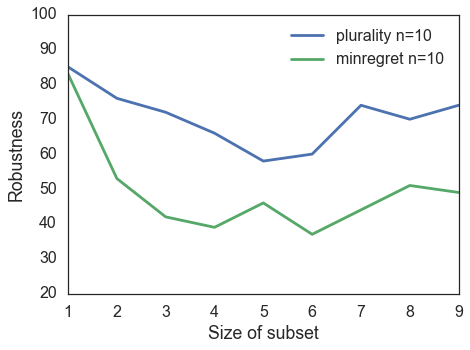
\includegraphics[height=4cm]{images/robustness_n10}
  \caption{Robustness with 10 voters and 10 choices}
  \label{fig:sub1}
\end{minipage}%
\begin{minipage}{.5\textwidth}
  \centering
  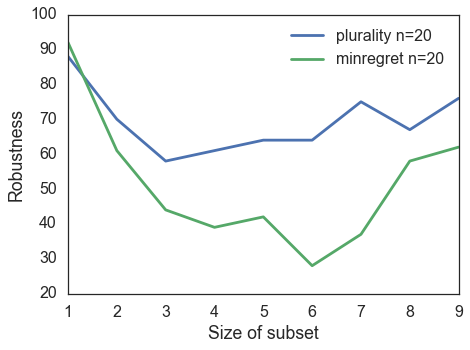
\includegraphics[height=4cm]{images/robustness_n20}
\caption{Robustness with 20 voters and 10 choices}\label{fig:sub2}
\end{minipage}
\end{figure}


We find that in general, plurality voting is much more robust to errors in voting than minimum regret. Then, based on our findings, we might expect that the additional cognitive load of ranking induces more errors in voting and that the algorithm is less robust to these errors.


%\subsection{Further Considerations}
%\citet{moulin2016handbook}  mentions four main considerations in evaluation of a voting rule. Communication cost, generality, and quality of the outcome have already been addressed above, in the sections concerning cognitive load, separability, and robustness, respectively. We now also touch briefly on the criterion of computational cost.

\section{Conclusion}
% More generally, even if the assumption of separability were to hold, it is not clear that utilitarian minimum regret should be the objective of choice in content aggregation. Minimum regret may in fact be a better aggregation function for meeting environments, when it is important that all participants have their needs addressed. However, for other content-based applications such as the construction of an argument as above or the composition of a Wikipedia-style article, perhaps it could make more sense to cater to the majority at the expense of minority opinions, depending on the target audience.
%% what happens to quality of outcome when assumptions do not hold
%% generality of approach

With respect to the general field of vote aggregation, our work suggests that the performance of various voting strategies depends on assumptions about separability and voting error. These assumptions seem to be violated. Future research should consider not only the performance of these algorithms given data, but also the effect of the corresponding data collection processes on the user experience.

Considering content aggregation specifically, we find that the ideal choice of utility and aggregation functions is likely environment-specific. In particular, even if the assumption of separability were to hold, it is not clear that utilitarian minimum regret should be the objective of choice in our content aggregation problem. Minimum regret may in fact be a better aggregation function for environments in which it is important that all participants have their needs addressed. However, for other content-based applications such as the construction of an argument as above or the composition of a Wikipedia-style article, perhaps it could make more sense to cater to the majority at the expense of minority opinions, depending on the target audience.


\section {Future work}
We have discussed how the separability of voting options and the cognitive load of the voting algorithm in question may confound results from a subset selection application where a crowd is asked to find a contextually relevant subset of points. Further research will involve understanding the impact of this context separability and outlining which scenarios should explicitly consider this factor. Moreover, work on cognitive load and voter fatigue (when ranking options, many participants made general placements of items as they were overwhelmed by the specifics of any one pairwise comparison)\footnote{See the third point in Appendix A} of the voting algorithm may help to shed light on the performance and stability of the voting schema.
%% explore contexts in which separability is/is not an issue?

% Note that plurality in many cases receives widespread critique as the winner in a voting rule may actually be highly unpopular \citep{moulin2016handbook}, however in the case of subset selection, the distance between different voting options may be small enough to neglect this downfall.

%\subsection{Citations}
%
%Here are two examples of how to cite a paper properly:
%\begin{itemize}
%	\item \citet{bernstein2000complexity} shows that ... 
%	\item Prior work has shown that ... \citep{bernstein2000complexity}.
%\end{itemize}


%%  \citet{key}  ==>>  Jones et al. (1990)
%%  \citep{key}  ==>>  (Jones et al., 1990)


%\section{Related Work}
%Discussion of previous important, similar work in the area with comparison to the particular approach taken and results of the paper. Avoid simply providing a laundry list of other work that is somehow related to the subject of the paper. This section should contain brief, in depth discussions of the work most similar to your project, i.e., to research that takes an approach to the problem or produces results with which your project should be compared. As is always the case with written work, throughout the paper you should have citations to work that you draw on. For example, if you have adapted a system, include a citation to the system when you first mention it; if you are extending a formalization, include a citation to the original on first mention. If you are unclear about whether a simple citation suffices or an extended discussion is needed in the Related Work section, look at the papers read for class this semester for models. If you are still unsure, check with the teaching staff.




%% The Appendices part is started with the command \appendix;
%% appendix sections are then done as normal sections
%% \appendix

%% \section{}
%% \label{}

%% References
%%
%% Following citation commands can be used in the body text:
%%
%%  \citet{key}  ==>>  Jones et al. (1990)
%%  \citep{key}  ==>>  (Jones et al., 1990)
%%
%% Multiple citations as normal:
%% \citep{key1,key2}         ==>> (Jones et al., 1990; Smith, 1989)
%%                            or  (Jones et al., 1990, 1991)
%%                            or  (Jones et al., 1990a,b)
%% \cite{key} is the equivalent of \citet{key} in author-year mode
%%
%% Full author lists may be forced with \citet* or \citep*, e.g.
%%   \citep*{key}            ==>> (Jones, Baker, and Williams, 1990)
%%
%% Optional notes as:
%%   \citep[chap. 2]{key}    ==>> (Jones et al., 1990, chap. 2)
%%   \citep[e.g.,][]{key}    ==>> (e.g., Jones et al., 1990)
%%   \citep[see][pg. 34]{key}==>> (see Jones et al., 1990, pg. 34)
%%  (Note: in standard LaTeX, only one note is allowed, after the ref.
%%   Here, one note is like the standard, two make pre- and post-notes.)
%%
%%   \citealt{key}          ==>> Jones et al. 1990
%%   \citealt*{key}         ==>> Jones, Baker, and Williams 1990
%%   \citealp{key}          ==>> Jones et al., 1990
%%   \citealp*{key}         ==>> Jones, Baker, and Williams, 1990
%%
%% Additional citation possibilities
%%   \citeauthor{key}       ==>> Jones et al.
%%   \citeauthor*{key}      ==>> Jones, Baker, and Williams
%%   \citeyear{key}         ==>> 1990
%%   \citeyearpar{key}      ==>> (1990)
%%   \citetext{priv. comm.} ==>> (priv. comm.)
%%   \citenum{key}          ==>> 11 [non-superscripted]
%% Note: full author lists depends on whether the bib style supports them;
%%       if not, the abbreviated list is printed even when full requested.
%%
%% For names like della Robbia at the start of a sentence, use
%%   \Citet{dRob98}         ==>> Della Robbia (1998)
%%   \Citep{dRob98}         ==>> (Della Robbia, 1998)
%%   \Citeauthor{dRob98}    ==>> Della Robbia


%% References with bibTeX database:

\section{References}
\bibliographystyle{elsarticle-num-names}
\bibliography{bibliography}

\appendix
\section{Qualitative Feedback from Survey}\label{appendix:qual_feedback}
\begin{itemize}
\itemsep0em 
\item \footnotesize Ranking was quite challenging, especially given that several statements were highly similar or conceptually related. I think it would be helpful to have some very stupid arguments thrown in so that you can have greater variability in your measurement. Glad to see you taking an interest in social psychology, little sister!
\item \footnotesize ranking is difficult, scoring and/or selecting is easier
\item \footnotesize Ticking the 5 most relevant points to support my argument is the easiest form of feedback. Placing the different points in order is the most difficult and requires the most time as you have to read through each point multiple times in order to make comparisons and form the list in the order you want. Ranking the points on a scale of 1-10 is also relatively easy, but may not give the most accurate results as I often just end up choosing a random number in the region of important (6-10) or unimportant (which in this case I just left as 1 as I had 5 points already).
\item \footnotesize I liked the first metric (separate scores) most, because I didn't have to do any artificial ranking or make difficult decisions between N things at once. I could. This is interesting though. One factor that will complicate your analysis is that more of the arguments for the first position were compelling than for the second two (though perhaps I'm biased by the format). So direct quantitative comparison between the formats, which doesn't account for the inherent differences in the distribution of argument persuasivenesses, might be misleading.
\item \footnotesize Selection was easiest to complete, but I think the rank-ordering will be the most highly informative.
\item \footnotesize Giving a score of 1 to 10 was the most difficult as it was hard to be fair and determine what I thought deserved a certain number. Choosing the 5 best arguments was fairly easy as I didn't really need to rank the statements. Dragging to rank all the choices was somewhat difficult but visually it was simple and easy because I was able to see my choices in order, rather than just attributing them a number 1 through 10.
\item \footnotesize Ranking is the most difficult.  I prefer the format that lets me choose on a scale from 1-10 how strong I think the argument is.  
\item \footnotesize Assigning values from 1-10 was the most difficult voting format.  Simple selection was the easiest, and ranking fell in the middle.  I believe simple selection will produce the most coherent points, but it may be a very small difference between ranking and selection.  Assigning values, while probably being better to analyze statistically, will probably produce the worst bias.
\item \footnotesize I think ranking was the easiest format in this survey
\item \footnotesize The checkbox question was the easiest to complete. The ranking question took the longest - I put greater emphasis on the first 5 ranks and cared less about the remaining 5. In the coring question from 1-10 I felt  that my numbers were fairly arbitrary and I did not need to use the full 1-10 scale (only used scores 1,5,6,7,8,9). 
\item \footnotesize 2/3rds of everything is irrelevant. What matters I suppose is being able to justifiably argue your point in a way which will support the evidence that preceded. Furthermore question the obvious and simply do what you can with what you have in the time you have left (desperado)
\item \footnotesize Question 1's ranking scheme was the easiest as it's easier to visually arrange points. However, Question 2's ranking scheme might produce a better sub-selection of 5 because the focus was on finding only the most relevant points (minimizing cognitive load a bit). 
\item \footnotesize Ranking was more difficult than selection. The selection will result in the most coherent sub-selection of 5 points. The constraint of only choosing the 5 most relevant points necessitates the person to do some sort of ranking. I like the simplicity of selecting the 5 points (the third format presented), but my preferred format of scoring each point from 1 to 10. This allowed me to assign 1 to the points I would never use and also put together a list of the points I would use in my debate. Furthermore, the usable points are now ranked in order, which may be handy when selecting points in a debate.
\item \footnotesize Ranking was more difficult. Particularly when needing to evaluate several equally poor statements, needing to determine an ordering among those was not as easy as simply assigning a score to each statement. I believe that the scoring mechanism will allow you to see definitive separation between stronger and weaker statements as the gap between their position/score can be demonstrably widened.
\item \footnotesize Was confusing that the first two questions went in opposite directions - easy to miss
\item \footnotesize I thought ranking the options (Question 3) was the best approach for comparing arguments. It's easier and faster to compare a given argument with two or one adjacent arguments than it is to judge them in absolute terms. I think the formats in Questions 2 and 3 are probably equivalent for selecting the best subset of five arguments. I disliked the format in Question 1 because it requires more work to compare different arguments. 
\item \footnotesize the drag-and-drop method facilitates focus on comparing two points when I repeatedly ask myself `is this option better than the one above it?' whereas the `select top 5' makes me compare the option in question to up to 5 others (if I've already selected 5) to decide if it deserves to be selected above one of the others; and the `rate each option' voting mechanism forces me to weigh up the relative strength of each option against all the other options in order to balance my scoring. 
\item \footnotesize Several theorems in game theory and social science [Arrow's, Gibbard�Satterthwaite] state that there's no excellent method of taking preferences from the members of a group and building a set of preferences (or single top choice) that the group would agree with. There might be a loophole around `separate into a top half and a bottom half', but it seems unlikely. Whatever mechanism you decide on will be vulnerable to some particular set of participant votes. That said, it may be possible to find a mechanism that works well for common voting patterns. It's also not clear why collecting LESS data (ordinal or top-5) would ever be more useful than collecting the full scores, unless perhaps the task of scoring 1-10 is more noisy for reasons of cognitive load and greater breaking of IIA. But certainly whatever math is run on the top-5 data could instead be run on the top 5 of the ranking data. Unless the aim of this research is to show that less taxing question formats are less noisy, I don't see the point. Overall, I suspect that I'm about to click through and get told I've been lied to and the real purpose of this research is something else altogether. 
\item \footnotesize I liked the voting format that automatically resorted the choices as they were selected. This made it visually easy to follow the order of 10 items and reorder as needed. I also liked the `choose the best 5' voting format, because I didn't have to select options that I felt were irrelevant, and also because I didn't have to put them in an order and found many choices to be equally as good as another. It was also quick and easy. I disliked the `insert order' voting option because it was cumbersome to go back and re enter numbers and ensure I didn't rank multiple options with the same number. I liked it better when it resorted for me..
\item \footnotesize Drag drop provides the most feedback -- you can immediately see the other items reordered. 
\item \footnotesize I found that question 1 required a fair amount of previous understanding of the US college application process and of acronyms used (such as ACT). I wasn't clear on what a few of the statements meant, not being familiar with the US system myself. I found selecting 5 relevant points the easiest selection, probably because I didn't need to have organized my thoughts as much as the first two that required specific ranking or scoring. I therefore believe that the relevant selection will probably result in the most whereby subsection of 5 points :)
\item \footnotesize I thought tanking was a bit more difficult. Trying to assess the strength of a single sentence set of claims based on a value of 1-10 is arbitrary. I thought it was a fascinating way to ask questions and fruitful to uncover interesting dynamics in the way that questions are answered.
\end{itemize}
% \appendix
\section{Question Topics}\label{appendix:question_topics}
\subsection{Topic 1:}
\textit{Many people feel that USA college admissions are highly skewed toward outdated metrics. Recent research has uncovered metrics that are better able to predict students' future performance in college. However, colleges are reluctant to adopt these new metrics.} Imagine that you are in a debate and you are asked to support the argument that USA college admissions should change their admission metrics.

\subsection{Topic 2:}
\textit{The `get to know you' styled interview is becoming a popular trend. However, research shows that humans are surprisingly bad at inferring essential qualities about an applicant's character and thus may make poor judgments about the future success of an applicant.} Imagine that you are in a debate and that you are asked to argue in support of the motion above, that the current structure of interviews is not helpful in successful hiring practices.


\subsection{Topic 3:}
\textit{The World Health Organization (WHO) has proposed to have video game addiction included in its catalog of mental diseases, but rhetoric stating that video games are addictive and comparing them to drugs is misguided.} Imagine that you are in a debate and that you are asked to support the statement that video games should not be classified as addictive.


\end{document}

